\documentclass[review]{vgtc}

\graphicspath{{figures/}{pictures/}{images/}{./}}

% Keep the VR template's metrics and line spacing; only add Unicode/CJK fonts.
\usepackage{times}
\renewcommand*\ttdefault{txtt}
\usepackage{mathptmx}
\usepackage{fontspec}
\usepackage{xeCJK}
\setmainfont{Times New Roman}
\setsansfont{Arial}
\setmonofont{Courier New}
\setCJKmainfont[BoldFont=SimHei,ItalicFont=KaiTi]{SimSun}
\setCJKsansfont{Microsoft YaHei}
\setCJKmonofont{FangSong}

\usepackage{amsmath}
\usepackage{amssymb}
\usepackage{enumitem}
\hyphenation{Ego-Anchor}
\usepackage{array}
\usepackage{booktabs}
\usepackage{multirow}
\usepackage{tabularx}
\usepackage{xcolor}
\usepackage{placeins}

\onlineid{1118}
\vgtccategory{System}
\vgtcinsertpkg

% XeLaTeX/xdvipdfmx 下禁用嵌套链接，避免官方模板的脚注正文丢失。
\hypersetup{nesting=false}

% 仅将 URL 改为接近官方模板的窄体等宽字体，避免脚注地址过度换行。
\newfontfamily\EgoUrlMono{Latin Modern Mono}
\renewcommand{\UrlFont}{\EgoUrlMono}

\title{EgoAnchor：透视混合现实中日常物体的零样本动态锚定}

\author{%
  Hailin Ji 
  \thanks{e-mail: \texttt{jihailin@mail.bnu.edu.cn}} \\
  School of Artificial Intelligence \\
  Beijing Normal University \\
  Beijing, China
  \and Yifeng Chen 
  \thanks{e-mail: \texttt{yfchen@mail.bnu.edu.cn}} \\
  School of Artificial Intelligence \\
  Beijing Normal University \\
  Beijing, China
  \and Haonian Wang
  \thanks{e-mail: \texttt{haonianwang@mail.bnu.edu.cn}} \\
  School of Artificial Intelligence \\
  Beijing Normal University \\
  Beijing, China
  \and Yiran Zhang 
  \thanks{e-mail: \texttt{zhangyiran@mail.bnu.edu.cn}} \\
  School of Artificial Intelligence \\
  Beijing Normal University \\
  Beijing, China
  \and Juyin Liu 
  \thanks{e-mail: \texttt{juyinliu@mail.bnu.edu.cn}} \\
  School of Artificial Intelligence \\
  Beijing Normal University \\
  Beijing, China
  \and Hongwen Zhang 
  \thanks{Corresponding author; e-mail: \texttt{zhanghongwen@bnu.edu.cn}} \\
  School of Artificial Intelligence \\
  Beijing Normal University \\
  Beijing, China
  \and Yanhong Luo 
  \thanks{Corresponding author; e-mail: \texttt{273961431@xbmu.edu.cn}} \\
  College of Electrical Engineering \\
  Northwest Minzu University \\
  Lanzhou, China
}

\abstract{%
零样本六自由度（6-DoF）物体位姿估计使未见日常物体的定位成为可能。然而，其输出具有异步、低频且质量波动的特征，难以直接作为透视混合现实（PMR）中连续、稳定的空间锚点。本文提出 EgoAnchor，一套第一人称零样本动态物体锚定系统。感知后端输出带视觉一致性评分的相机系位姿观测；运行时将其转换为图像采集时刻的世界系状态，并维护可靠的对象状态，从而生成连续、稳定且支持遮挡恢复的锚点。我们在 Meta Quest 3 上实现系统，并通过以平台跟踪控制器为参考的受控基准测试、关键模块消融和 24 名被试的被试内实验进行评估。相较基准方法，EgoAnchor 的静态配准误差、遮挡恢复误差和时延对齐轨迹残差更低，但运动响应时延更高；主观实验显示，其虚实融合感、交互信任度和依赖意愿评分更高。系统源代码将在录用后开源。
}

\keywords{透视混合现实, 动态物体锚定, 6-DoF 位姿估计, 运行时系统, 用户感知}

% ===== Teaser =====
\teaser{%
  \centering
  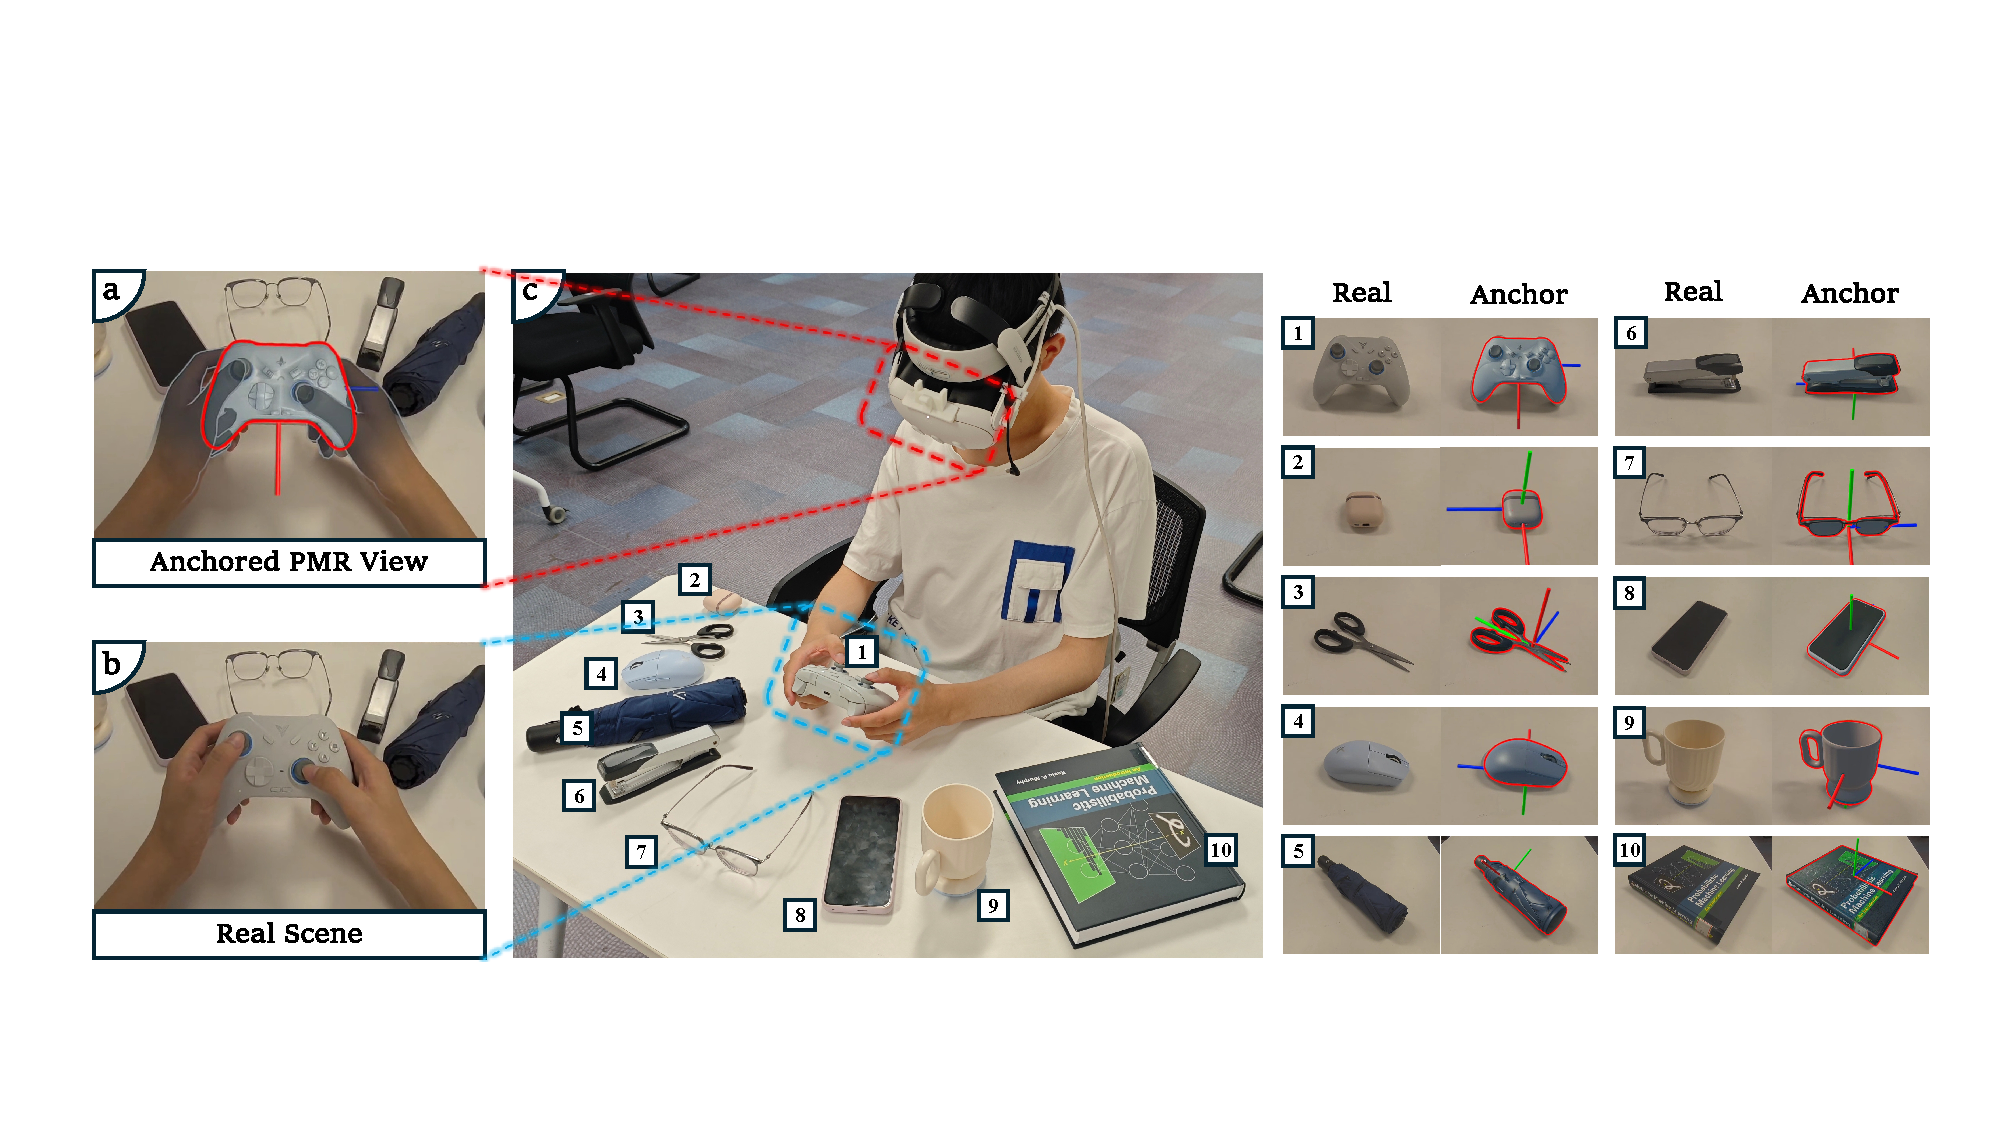
\includegraphics[width=\linewidth]{figures/teaser.pdf}
  \caption{EgoAnchor 在日常物体上的零样本动态锚定示例：(a) 第一人称锚定增强画面；(b) 同一时刻未增强的透视画面；(c) 第三人称交互视角。场景编号 1--10 与右侧十个物体对应；每组展示真实物体（Real）与 EgoAnchor 锚定可视化（Anchor）。红色轮廓与局部坐标轴表示估计的 6-DoF 对象锚点。十个物体依次为游戏手柄、耳机盒、剪刀、无线鼠标、雨伞、订书机、眼镜、手机、马克杯和书本，覆盖不同尺度、几何与外观。}
  \label{fig:teaser}
}

\begin{document}

\firstsection{引言}\label{sec:introduction}
\maketitle

% ===== 第一段：问题动机 =====
透视混合现实（Passthrough Mixed Reality, PMR）支持将虚拟内容附着于真实物体，用于操作说明、交互引导、状态可视化与近物交互。此类应用需随物体运动持续维护对象级空间参考：在用户头动、操纵物体或短暂遮挡时，虚拟叠加层仍应保持相对于物体一致的六自由度（6-DoF）变换。传统空间锚点面向静态环境，无法表达物体自身运动；因此，动态对象锚定是以物体为中心的 MR 应用的一项基础能力~\cite{selfblending2026,gradualreality2024}。

% ===== 第二段：现有方案局限 =====
现有方案在不同技术层面提供了部分支持。商用头显原生提供的对象跟踪接口集成度高，但其支持的对象类别、几何模型要求与运行时行为受平台特定定义限制（如 Apple Vision Pro 与 Meta Quest 系列）；物理标记（如 AprilTag、ArUco）与专用硬件跟踪器（如 HTC Tracker）能够提供稳定定位，但必须预先改造目标物体或安装附加硬件。近年来，开放词表检测、时序分割、双目立体匹配与模型驱动的零样本 6-DoF 位姿估计为具有已知三维模型的刚性物体提供了视觉定位能力~\cite{groundingdino2025,cutie2024,fastfoundationstereo2026,foundationpose2024,gigapose2024}。这些感知基础模型拓展了视觉定位的适用范围，但其输出本质上仍是与特定图像采集时刻绑定的离散、异步相机系观测，无法直接提供可供 MR 内容稳定绑定的对象锚点。

% ===== 第三段：核心问题 =====
直接采用视觉位姿作为对象锚点会引入若干关键问题。首先，异步结果到达渲染端时已累积时延；若与到达时刻的相机位姿复合，头动会被误作物体运动。其次，候选位姿仍可能因遮挡、深度噪声或几何错配而跳变，直接接纳会引发渲染抖动。最后，低频、不规则的含噪位姿流无法匹配高频渲染，运行时还需管理静止、运动、短时失效与重新获取。因此，单帧位姿估计不足以形成持续可用的对象锚点。

% ===== 第四段：EgoAnchor解决方案 =====
本文提出 EgoAnchor，一套第一人称零样本动态物体锚定系统。感知后端将开放词表检测、时序分割、双目深度恢复与零样本位姿估计组织为连续流水线，并采用逐观测可视度门控颜色--深度评分（Visibility-gated Color-Depth, VCD）评估可靠性。运行时将异步候选转换为采集时刻的世界系观测，维护面向实时渲染的可靠对象状态，并在物体运动、静止和短时观测中断期间生成连续可用的空间锚点。对于新目标物体，无需物理标记或逐物体训练，仅需三维模型与简短文本描述；三维模型可采用已有数字资产，或由图像离线重建获得。

% ===== 第五段：贡献 =====
本文的主要贡献为：
\begin{enumerate}[leftmargin=1.8em,itemsep=1pt,topsep=2pt]
  \item \textbf{EgoAnchor 系统：}将异步、低频且质量波动的相机系零样本视觉观测转化为连续可用的世界系动态对象锚点。
  \item \textbf{面向锚定的感知与运行时：}采用 VCD 评估逐观测可靠性，并通过采集时刻对齐、时间索引轨迹与静止锁定维持连续、可恢复的运行时输出。
  \item \textbf{系统评估：}通过以平台跟踪控制器为参考的受控基准测试、关键模块消融与 24 名被试的被试内用户实验，量化系统性能、设计取舍及用户感知。
\end{enumerate}

\section{相关工作}\label{sec:related-work}

\subsection{MR 物体锚定}

物体锚定为真实物理实体建立空间参考，使虚拟内容持续附着并跟随物体。早期方法依赖 AprilTag、ArUco 等人工标记解算位姿~\cite{apriltag2011,aruco2014}，需改造目标物体，难以覆盖开放场景。

商业 MR 生态中已出现多种免标记对象识别与跟踪方案。Azure Object Anchors（已于 2024 年退役）\footnote{\href{https://learn.microsoft.com/en-us/lifecycle/end-of-support/end-of-support-2024}{Azure Object Anchors retirement}}、Vuforia Model Targets\footnote{\href{https://developer.vuforia.com/library/vuforia-engine/images-and-objects/model-targets/model-targets/}{Vuforia Model Targets}}、Apple Vision Pro\footnote{\href{https://developer.apple.com/documentation/visionos/implementing-object-tracking-in-your-app}{Apple object tracking}} 和 Meta Quest\footnote{\href{https://developers.meta.com/horizon/documentation/native/android/mobile-dynamic-object-tracker/}{Meta dynamic object tracking}} 均借助设备感知与目标模型估计对象状态。这些方案通常依赖专有对象扫描或离线配置，并受对象类型与平台接口限制。学术研究进一步结合头显跟踪、空间映射、相机与深度感知，实现资产定位、已知物体注册和持续跟踪~\cite{fan2021assettracking,doughty2022hmdegopose,pollabauer2023hololens,martingomez2024sttar,trojak2025mixedpose,greene2025markerless,trojak2026markerless,gbot2024}，但仍常依赖特定对象、任务先验、专用硬件或平台配置，对开放场景中多类日常物体的灵活接入支持有限~\cite{hurt2025surrealitycv}。

\subsection{6-DoF 物体位姿估计与跟踪}

6-DoF 位姿估计从视觉观测恢复刚性物体的相机系位姿，是动态锚定的感知基础~\cite{aguirrezabal2026survey}。研究已从局部特征匹配发展到利用 RGB-D 融合、稠密几何回归、对称性建模和自监督学习的已知实例估计~\cite{densefusion2019,epos2020,gdrnet2021,self6d2020}，并扩展到未见物体与零样本场景~\cite{gen6d2022,megapose2022,lin2024sam6d,ornek2024foundpose,moon2025coop,foundationpose2024}；粒子滤波与多帧几何约束则可维持跨帧状态~\cite{poserbpf2021,bundletrack2021}。

视觉基础模型进一步扩大了开放场景感知范围：开放词表检测器根据自然语言描述定位目标~\cite{owlvit2022,glip2022,groundingdino2025,yoloe2025}，视频对象分割模型沿时间传播目标身份与轮廓~\cite{xmem2022,cutie2024}，现代双目立体匹配则提升了复杂场景下的深度恢复与跨域泛化~\cite{raftstereo2021,igevstereo2023,fastfoundationstereo2026}。这些能力使日常物体的零样本定位逐渐可行，但主要解决相机系局部感知；在 MR 中，观测仍需转化为稳定、连续的世界系对象状态。

\subsection{XR 时间对齐}

XR 的图像采集、推理与传输会引入且动态改变端到端时延，使渲染状态对应于更早的观测~\cite{diluca2010latency,mrloop2022,stauffert2020mtp}。针对状态时间戳与显示目标时刻之间的错位，一类典型方法是\emph{预测跟踪（predictive tracking）}：依据历史运动模型将状态外推至当前或预期显示时刻，以减小动态配准误差~\cite{azuma1994improving,laviola2003double,pvt2023,yoon2022headmotion}。

另一种方法保留带时间戳的状态记录，按历史时刻查询或插值重建状态。AR 系统已通过时间戳同步、采样调整及插值或外推重配准异构时延数据流~\cite{jacobs1997latency}。OpenXR\footnote{\href{https://registry.khronos.org/OpenXR/specs/1.1/man/html/xrLocateSpace.html}{OpenXR xrLocateSpace}} 也区分未来状态预测与\emph{历史状态查询（history query）}：前者减小相位滞后，后者恢复过去时刻的空间几何状态。

\section{EgoAnchor 系统}\label{sec:system}

\subsection{系统概述}

EgoAnchor 以文本描述与离线三维模型指定目标，无需物理标记或逐物体训练。感知后端生成带可靠性评分的相机系位姿，运行时将其转换为采集时刻的世界系位姿，并按渲染时钟维护锚点。

运行时区分图像采集时刻 $t_f$、候选到达时刻 $t_a$ 与渲染时刻 $t_r$。以 $T_a^b\in\mathrm{SE}(3)$ 表示将坐标从坐标系 $a$ 映射至坐标系 $b$ 的刚体变换；$w,c,o$ 分别表示世界、左目相机与对象局部坐标系，$\widehat{T}$ 与 $\widetilde{T}$ 则分别表示滤波状态与应用输出。图~\ref{fig:arch}展示系统架构。

\begin{figure*}[t]
  \centering
  
\includegraphics[width=\textwidth]{figures/pipeline.pdf}
  \caption{EgoAnchor 架构与异步数据流。感知后端根据双目图像、文本描述和三维模型完成语义初始化、时序分割、深度恢复与零样本 6-DoF 位姿估计，并根据可视度（V）、颜色（C）和深度（D）计算 VCD 可靠性。异步观测 $o_f$ 到达运行时后按采集时刻转换为世界系位姿，经准入与状态更新形成时间索引轨迹 $B_j$；渲染帧 $t_r$ 在 $t_q$ 查询轨迹，并在动态跟踪与静止锁定之间切换。可靠观测持续缺失时触发重新获取。}
  \label{fig:arch}
\end{figure*}

\subsection{感知后端}\label{sec:perception}

\textbf{输入与观测表示。}
给定双目图像 $I_f = (I_f^L, I_f^R)$、目标描述 $Q_o$ 与三维模型 $G_o$，后端为每个处理帧形成观测：
\begin{equation}
o_f = (f, t_f, T_{o,f}^{c}, R_f),
\label{eq:observation}
\end{equation}
其中 $f$ 为单调递增帧标识，$T_{o,f}^{c}$ 为目标在左目相机坐标系中的 6-DoF 位姿，$R_f \in [0,1]$ 为可靠性评分；$\{o_f\}$ 构成异步观测流。

\subsubsection{面向锚定的感知流水线}

流水线依次建立目标身份、度量深度与相机系位姿。

\textbf{语义初始化。}
开放词表检测器~\cite{yoloe2025}在初始化帧 $f_0$ 由左目图像与文本描述获得目标分割掩膜：
\begin{equation}
M_{f_0} = \operatorname{Detect}(I_{f_0}^{L}, Q_o),
\label{eq:detect}
\end{equation}
其中 $f_0$ 为首次同时获得有效掩膜与足够深度覆盖的帧；重新获取时系统重置 $f_0$。

\textbf{时序分割。}
初始掩膜用于初始化视频对象分割网络~\cite{cutie2024}，此后逐帧传递目标时序身份：
\begin{equation}
(M_f, H_f) = \operatorname{Seg}(I_f^{L}, H_{f-1}), \qquad f > f_0,
\label{eq:seg}
\end{equation}
其中 $H_f$ 为用于维持同一目标实例身份的时序外观记忆。

\textbf{双目深度恢复。}
立体匹配网络由校正后的双目图像预测视差并恢复米制深度：
\begin{equation}
d_f = \operatorname{Stereo}(I_f^{L}, I_f^{R}), \qquad Z_f = \frac{b f_x}{d_f},
\label{eq:depth}
\end{equation}
其中 $b$ 与 $f_x$ 分别为双目基线距离和像素焦距。

\textbf{零样本位姿估计。}
模型驱动估计器~\cite{foundationpose2024}由掩膜、深度与三维模型恢复相机系位姿：
\begin{equation}
T_{o,f}^{c} =
\begin{cases}
\operatorname{Reg}(M_f, Z_f, G_o), & \text{注册}, \\
\operatorname{Track}(M_f, Z_f, G_o, T_{o,f^-}^{c}), & \text{跟踪}.
\end{cases}
\label{eq:pose}
\end{equation}
全局注册仅用于初始化与重新获取；连续帧以前一结果初始化局部跟踪。

\subsubsection{逐观测 VCD 评分}

局部遮挡或噪声可能使零样本位姿候选与图像证据不一致。VCD 将理论渲染结果与对应观测进行比较~\cite{deepim2018,latentfusion2020,focalpose2022}，结合可视度（V）、颜色（C）与深度（D）评估候选可靠性。

\textbf{可视度门控。}
记 $M_f^{\mathrm{rnd}}$ 为候选位姿下的理论渲染掩膜，定义：
\begin{equation}
\Omega_f = M_f \cap M_f^{\mathrm{rnd}}, \quad \Omega_f^{\circ} = \operatorname{Erode}(\Omega_f), \quad V_f = \frac{|\Omega_f|}{|M_f^{\mathrm{rnd}}|},
\label{eq:visibility}
\end{equation}
其中 $V_f$ 为渲染投影受观测掩膜支持的比例；腐蚀区域 $\Omega_f^\circ$ 减小边缘混合像素影响。

\textbf{颜色与深度一致性。}
颜色一致性 $S_f^C$ 采用 CIE $L^*a^*b^*$ 颜色空间内的零均值归一化互相关（ZNCC），并降低明度通道的权重。深度一致性结合距离自适应绝对残差项 $S_f^{D,\mathrm{abs}}$ 与对整体深度系统偏差较鲁棒的表面法向结构项 $S_f^{D,\mathrm{str}}$：
\begin{equation}
S_f^D = (1-\alpha_f)\,S_f^{D,\mathrm{abs}} + \alpha_f\,S_f^{D,\mathrm{str}}.
\label{eq:depth-score}
\end{equation}
其中 $\alpha_f$ 由局部深度变化确定，使平坦目标侧重绝对深度、几何起伏目标侧重局部结构。

\textbf{证据聚合。}记 $K_f\subseteq\{C,D\}$ 为本帧有效模态集合，则综合评分定义为：
\begin{equation}
R_f = V_f \cdot
\begin{cases}
\exp\!\left(\dfrac{\sum_{k \in K_f} w_k \ln \max(S_f^{k}, \epsilon)}{\sum_{k \in K_f} w_k}\right), & K_f \neq \varnothing, \\[6pt]
1, & K_f = \varnothing,
\end{cases}
\label{eq:vcd}
\end{equation}
其中 $w_k$ 为模态权重，$\epsilon$ 避免对数奇异。无效模态不参与聚合；颜色与深度均不可用时，评分退化为 $V_f$。乘性门控使严重遮挡或投影错位直接降低可靠性。

\subsection{锚定运行时}\label{sec:anchoring}

运行时将低频异步候选转化为显示同步的对象状态：候选到达时转换为采集时刻的世界系位姿并更新轨迹，渲染帧通过插值合成锚点，并管理静止锁定与有效性。候选与渲染事件解耦，使输出频率不受推理速率限制。

\subsubsection{观测校正}\label{sec:obs-update}

运行时将候选转换为采集时刻的世界系位姿，经可靠性与时序准入后更新轨迹。

\textbf{观测对齐。}
候选 $T_{o,f}^{c}$ 对应采集时刻 $t_f$，但在 $t_a$ 返回；与到达时刻的相机位姿复合会将期间的头动引入对象位姿。运行时按帧标识 $f$ 检索缓存的 $T_{c,f}^{w}$，并计算：
\begin{equation}
T_{o,f}^{w} = T_{c,f}^{w}
\begin{bmatrix}
1 & 0 & 0 & 0 \\
0 & -1 & 0 & 0 \\
0 & 0 & 1 & 0 \\
0 & 0 & 0 & 1
\end{bmatrix}
T_{o,f}^{c}
\begin{bmatrix}
-1 & 0 & 0 & 0 \\
0 & 1 & 0 & 0 \\
0 & 0 & 1 & 0 \\
0 & 0 & 0 & 1
\end{bmatrix}.
\label{eq:capture-alignment}
\end{equation}
其中左、右两个固定矩阵分别转换相机坐标系与对象局部坐标系，以处理视觉系统和渲染系统轴向约定的差异。

\textbf{可靠准入。}
第 $j$ 个接纳观测记为 $(t_j,T_{o,j}^{w},R_j)$。首个候选满足可靠性门槛即可建立轨迹，后续候选还须时刻递增：
\begin{equation}
R_f \geq R_{\min}, \qquad t_f > t_j \quad (j \geq 1).
\label{eq:admission}
\end{equation}
未通过准入条件的候选不更新内部状态。

\textbf{状态更新。}
每个接纳观测触发平移与旋转的常速度卡尔曼滤波更新~\cite{kalman1960new}，得到滤波状态 $\widehat{T}_{o,j}^{w}$ 及时间索引轨迹：
\begin{equation}
B_j = \{(t_i, \widehat{T}_{o,i}^{w})\}_{i=1}^{j}.
\label{eq:trajectory}
\end{equation}
该更新同时刷新静止锁定机制所需的运动与可靠性指标。

\subsubsection{锚点合成}\label{sec:frame-output}

轨迹 $B_j$ 低频且间隔不规则。运行时先确定历史查询时刻 $t_q$，再由相邻节点插值生成逐帧状态。

\textbf{历史查询。}
最新可用节点时刻 $t_j$ 相对渲染时刻 $t_r$ 的状态年龄为 $\ell_r=t_r-t_j$，运行时根据其非对称指数平滑估计 $\bar{\ell}_r$ 动态设置查询滞后量：
\begin{equation}
\ell_r = t_r - t_j, \qquad \Delta_r = \max(\Delta_{\min},\, s\,\bar{\ell}_r), \qquad t_q = t_r - \Delta_r.
\label{eq:target-time}
\end{equation}
其中 $\Delta_{\min}$ 为最小查询滞后，$s$ 为缩放因子；该策略提高 $t_q$ 位于两个已到达节点之间的概率。

\textbf{状态插值。}
当查询时刻满足 $t_i\leq t_q\leq t_{i+1}$ 时，运行时在相邻轨迹节点之间对物体位姿进行几何插值：
\begin{equation}
\lambda_q = \frac{t_q - t_i}{t_{i+1} - t_i}, \qquad
\widehat{T}_o^w(t_q) = \operatorname{Interp}(\widehat{T}_{o,i}^{w}, \widehat{T}_{o,i+1}^{w}; \lambda_q).
\label{eq:history-interp}
\end{equation}
位置采用线性插值（LERP），旋转采用四元数球面线性插值（SLERP）；超出轨迹区间时保持最近端点状态。

\textbf{输出模式。}为抑制静止期的微幅扰动，EgoAnchor 在动态跟踪与静止锁定之间自适应切换：
\begin{equation}
\widetilde{T}_o^w(t_r) = \begin{cases}
\widehat{T}_o^w(t_q), & \text{跟踪}, \\
T_{o,\mathrm{lock}}^w, & \text{锁定}.
\end{cases}
\label{eq:staticlock}
\end{equation}

\subsubsection{静止锁定}\label{sec:staticlock}

本文将该静止状态锚定机制定义为 \emph{StaticLock}：在持续低运动且观测可靠时切换为锁定位姿，检测到明确运动或可靠性下降时平滑解除锁定。

\textbf{进入。}由相邻接纳观测解算并指数平滑平移与旋转速率 $\bar v_j,\bar\omega_j$，定义复合判定：
\begin{equation}
\max\left(\frac{\bar{v}_j}{v_{\mathrm{th}}},\ \frac{\bar{\omega}_j}{\omega_{\mathrm{th}}}\right) \leq 1, \qquad R_j \geq R_{\mathrm{lock}}.
\label{eq:lock-entry}
\end{equation}
条件持续 $\tau_{\mathrm{dwell}}$ 后，以当前跟踪位姿初始化 $T_{o,\mathrm{lock}}^w$，并冻结低通观测均值 $T_{o,\mathrm{ref}}^w$ 以度量累计漂移。

\textbf{锁定状态更新。}
设 $d_{p,j}$ 和 $d_{\theta,j}$ 分别表示当前观测与锁定位姿之间的平移和旋转残差。基于死区阈值 $d_{\mathrm{db}}$ 和 $\theta_{\mathrm{db}}$，定义归一化偏差 $\delta_j=\max(d_{p,j}/d_{\mathrm{db}},d_{\theta,j}/\theta_{\mathrm{db}})$。锁定位姿更新规则为：
\begin{equation}
T_{o,\mathrm{lock},j}^w =
\begin{cases}
\operatorname{Interp}\left(T_{o,\mathrm{lock},j-1}^w, T_{o,j}^{w};\, g_j\right), & \delta_j \leq 1, \\
T_{o,\mathrm{lock},j-1}^w, & \delta_j > 1.
\end{cases}
\label{eq:lock-update}
\end{equation}
其中 $g_j$ 为可靠性调节的微小增益。死区内漂移由阻尼更新吸收，超出死区的偏移用于触发解锁。

\textbf{释放。}当死区外残差持续存在、相对 $T_{o,\mathrm{ref}}^w$ 的漂移超限、检测到明确持续运动或可靠性骤降时，系统在下一渲染帧平滑退回跟踪模式；运动判据随头动强度适度放宽，以减少误释放。

\textbf{有效性与重新获取。}\label{sec:validity}
锚点按近期可靠观测标记为有效、不确定或丢失：短时缺失时继续查询轨迹并可保持最后可信位姿，超时后停止输出。锚点丢失或候选持续低可靠时，后端重新检测与注册并重置轨迹，由首个新接纳观测开启跟踪周期。

\section{系统实现}\label{sec:implementation}

EgoAnchor 的后端与运行时通过局域网通信。感知后端部署于配备 NVIDIA RTX 5090 GPU 的工作站，基于 Python 3.14.6、PyTorch 2.12.1、CUDA 13.2 与 TensorRT 11.1 实现；客户端运行时基于 Unity 6000.3.11f1 与 Meta XR SDK 203.0.0 构建，经 Quest Link 运行于配备 Intel i9-14900K 处理器及 32~GB 内存的主机。Meta Quest 3 负责双目透视采集、设备定位与渲染显示。

\textbf{感知后端。}
后端使用 YOLOE-26 初始化开放词表目标~\cite{yoloe2025}，使用 Cutie 传播目标掩膜~\cite{cutie2024}，使用 Fast-FoundationStereo 恢复米制深度~\cite{fastfoundationstereo2026}，并使用 FoundationPose 执行零样本 6-DoF 注册与局部跟踪~\cite{foundationpose2024}；VCD 借助 nvdiffrast 实现硬件加速的在线模型光栅化~\cite{nvdiffrast2020}。在 RTX 5090 配置下，跟踪阶段服务器端处理时间的中位数和 P95 分别为 75.44~ms 和 88.47~ms，候选到达率中位数为 13.25~Hz；后续定量实验均在该硬件环境下完成。

\textbf{锚定运行时。}
运行时以 C\# 实现，通过 Meta Passthrough Camera API 获取校正双目图像与相机标定参数，并以帧标识缓存相机位姿历史队列。所有运行时阈值与增益参数在三个评估实验中保持完全固定；完整参数清单随补充材料提供。

\textbf{通信。}
双目图像与相机标定数据通过 ZeroMQ 和 Protobuf 传输，并采用最新帧优先策略以抑制队列积压；6-DoF 位姿、系统状态与控制信令通过 NATS Core 消息总线传输。图像帧与返回观测保留一致的帧标识，供运行时检索对应采集时刻的相机位姿。

\section{评估设计}\label{sec:evaluation}

本文通过三个互补实验评估 EgoAnchor：实验一在受控条件下比较四种运行时配置的静态、动态与状态转换行为；实验二分别考察采集时刻对齐、静止锁定、VCD 可靠性排序以及预测跟踪与历史查询；实验三以日常刚性物体开展包含 24 名被试的被试内用户实验，考察主观锚定质量、虚实融合感、交互信任度与依赖意愿。

日常物体三维模型通过 Hunyuan3D\footnote{\url{https://3d.hunyuan.tencent.com/}}~\cite{hunyuan3d22025tencent} 由多视角手机照片生成，并经过网格轻量化与贴图烘焙处理；Quest 3 控制器采用官方标准数字资产。

\subsection{实验一：系统性能}\label{sec:exp1-design}

\textbf{参考与场景。}
评估以 Quest 3 控制器为视觉跟踪目标，并以平台 SDK 输出的 6-DoF 位姿作为跟踪参考。四类采集场景包括静止目标下的主动头动、静止与 6-DoF 运动之间的起停切换、连续空间平移与旋转，以及完全遮挡后的跟踪恢复，分别用于考察静态稳定性、状态转换响应、动态跟随与遮挡恢复性能。

\textbf{比较条件。}
四种配置接收相同的原始候选位姿流。\textbf{Arrival}/\textbf{Capture} 均保持最新候选，仅在转换至世界坐标系时分别使用到达时刻与采集时刻的相机位姿。\textbf{One-Euro}~\cite{casiez2012oneeuro} 作为实时交互系统中兼顾抖动抑制与低时延响应的代表性平滑基线，对接纳观测进行速度自适应低通滤波并维护时间索引轨迹，但不启用静止锁定。\textbf{EgoAnchor} 为本文的完整系统。

\textbf{评价指标。}
九项定量指标按系统响应特性分为三组。\textbf{静态配准}指标包括头动耦合误差（静止目标条件下由观察者头动引起的锚点空间偏移）、配准误差（相对于平台跟踪参考的空间偏差）和静止抖动（静止条件下相邻渲染帧之间的位姿变化）。\textbf{动态跟随}指标包括有效时延（使估计轨迹与参考轨迹的残差最小的时间偏移量）、LA-RMSE（时延对齐后的几何轨迹残差）、CT-RMSE（未进行时延对齐的当前时刻误差）以及残余抖动（时延对齐后残差中的高频分量）。\textbf{状态转换响应}指标包括遮挡恢复误差（从遮挡发生至跟踪恢复稳定期间的位姿偏差）和运动响应时延（从物体开始运动至锚点产生响应的时间间隔）。除运动响应时延作为跨通道标量统计外，其余指标均分别在平移和旋转通道上报告。

\subsection{实验二：消融分析}\label{sec:exp2-design}

实验二针对四项关键设计开展消融分析。

\textbf{观测对齐。}
同一相机系候选分别与图像采集时刻和候选到达时刻的相机位姿复合，比较主动头动条件下的头动耦合误差，以评估采集时刻对齐对静态配准的影响。

\textbf{静止锁定。}
在完整 EgoAnchor 上关闭静止锁定，比较静止条件下的头动耦合误差与抖动，以量化该模块对静止期锚点稳定性的贡献。

\textbf{VCD。}
候选按 VCD 评分由高到低排序，绘制风险--覆盖率曲线，并以曲线下面积（AURC）量化评分对几何误差的排序能力~\cite{riskcontrolled2020,ding2020uncertainty}；AURC 越低，表明高评分候选总体上具有越低的几何误差。

\textbf{预测与历史查询。}
为量化响应速度与轨迹保真度之间的权衡，我们对比\emph{预测跟踪}与\emph{历史状态查询}。前者基于经卡尔曼滤波的常速度模型外推至 $t_r$；后者按第~\ref{sec:frame-output}~节在 $t_q$ 对相邻轨迹节点执行平移线性插值与旋转 SLERP。两者共享相同的候选流、状态估计与准入规则。

\subsection{实验三：用户实验}\label{sec:exp3-design}

实验三进一步考察受控评价中的系统差异是否反映到用户主观感知。我们在日常刚性物体上对比 One-Euro 与完整 EgoAnchor，重点测量静止稳定性、运动附着、遮挡恢复以及用户对锚点的虚实融合感、交互信任度与依赖意愿。

\subsubsection{实验设计}

研究选取在视觉可观测性和操作遮挡方面具有互补特征的无线鼠标、订书机与游戏手柄，分别代表弱纹理曲面、细长多平面，以及具有丰富几何与纹理但易受自然抓握遮挡的物体。实验采用完全被试内设计，每位被试均在三个物体上体验 One-Euro 与 EgoAnchor；六个方法--物体条件采用平衡拉丁方排序，并以匿名 A/B 标签呈现，以降低顺序效应。

\subsubsection{任务}

每个方法--物体条件依次完成三项标准化操作：(1) 静止多角度观察；(2) 拿起物体完成约 25--30~cm 平移与 30--45° 自然旋转后放回；(3) 用统一挡板完全遮挡目标约 1~s 后移开并观察恢复过程。三项任务完成后进行主观量表评分。

\subsubsection{主观测量}

主观测量包括七项对象锚定条目，以及 Augmentation Quality（AQ）、Trust in Automation（TiA）和 S-TIAS 三个标准化量表。

\textbf{对象锚定条目。}
七项条目均采用七点同意度量表，覆盖实验一所考察的应用层行为，并参考已有 AR 跟踪与信任研究~\cite{trustar2024}：阶段行为包括静止稳定性、运动附着性、姿态一致性和恢复一致性，整体判断包括位置正确性、依赖意愿和稳定性--响应性权衡。各条目分别分析，完整措辞见补充材料。

\textbf{增强质量（AQ）。}
采用 AQ~\cite{aq2026} 的嵌入质量（EQ）与交互质量（IQ）两个完整三条目子量表，分别评价虚实融合感（几何嵌入）以及操作过程中的交互质量，均为七点量表。

\textbf{用户信任（TiA与S-TIAS）。}
TiA~\cite{tia2019} 采用可靠性/能力（6 项）与理解/可预测性（4 项）两个子量表（五点量表），S-TIAS~\cite{stias2025} 以三个七点条目评估总体交互信任度。量表仅对指代对象进行情境化适配，中文译文经逐条核对并在预实验中完成可理解性验证。

最终问卷另行记录总体方法偏好、信任选择、偏好强度、方法区分信心与实验后不适反馈，均作描述性报告。

\subsubsection{实验流程}

研究获得所属机构伦理审查委员会批准，被试在实验前签署知情同意书。在完成背景调查、头显穿戴调节与操作练习后，被试依次体验六个方法--物体条件，并在每个条件后完成对象锚定条目与 AQ 量表；全部条件结束后，被试分别评价两种方法的 TiA 与 S-TIAS，并填写最终问卷。单次实验时长约 60 分钟，其间允许被试按需休息。

\subsubsection{参与者}

共招募 24 名被试并全部纳入最终分析（年龄 20--36 岁，$M=27.08$，$\mathrm{SD}=4.45$；女性与男性各 12 名；22 名右利手）。其中 6 名从未使用过 VR/MR，10 名使用过 1--5 次，8 名使用过 6 次以上；12 名被试此前无真实物体 AR/MR 空间操作经验。

\subsubsection{统计分析}

对每名被试，七项对象锚定条目的各项得分与两个 AQ 子量表得分均先跨三个物体取均值；TiA 的两个子量表与 S-TIAS 则按方法分别计算条目均分，共形成 12 项结果。各指标报告中位数与四分位距 $\mathrm{Mdn}\ [\mathrm{Q}_1, \mathrm{Q}_3]$；24 组配对样本采用双侧 Wilcoxon 符号秩检验，并报告配对秩双列相关系数 $r_{\mathrm{rb}}$ 及其 95\% 置信区间。七项自定义条目与五项标准化量表分别构成两个独立的 Holm--Bonferroni 校正家族；量表内部一致性按方法报告 Cronbach's $\alpha$。

\section{结果}\label{sec:results}

\subsection{实验一：系统性能}

结果按第~\ref{sec:exp1-design}~节指标体系报告。表~\ref{tab:exp1-static}--\ref{tab:exp1-transition} 汇总了中位数统计量，图~\ref{fig:exp1-final} 展示多次重复实验的误差分布，图~\ref{fig:exp1-replay} 展示动态序列的连续回放。指标先在单次测试序列内汇总，再取多次重复间的中位数；平移与旋转通道分别独立报告。

\begin{figure*}[!t]
  \centering
  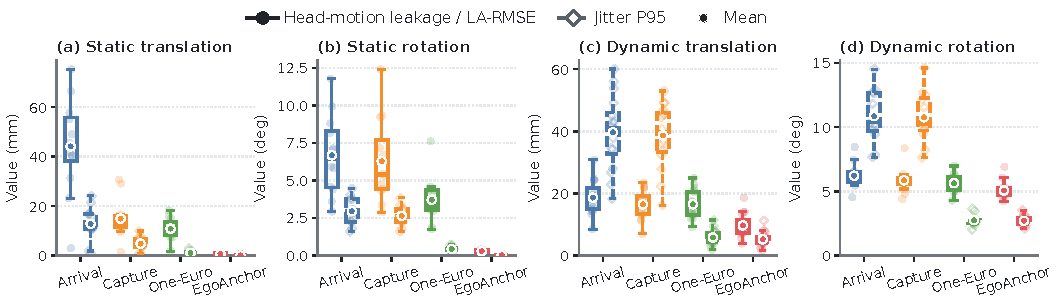
\includegraphics[width=\textwidth]{figures/panels/figure2_exp1_behavior.pdf}
  \caption{实验一四种配置的误差分布：(a,b) 静止状态下的平移与旋转通道，展示单次测量内头动耦合误差和静止抖动 P95 在多次重复间的分布；(c,d) 持续运动状态下的平移与旋转通道，展示 LA-RMSE 与单次测量内残余抖动 P95 在多次重复间的分布。每个浅色散点表示一次重复测量；箱体与中心线分别表示 IQR 与中位数，深色点表示均值。所有指标均为越低越好。}
  \label{fig:exp1-final}
\end{figure*}

\subsubsection{静态配准}

\begin{table}[t]
\centering
\caption{实验一静态配准指标。各单元格按平移/旋转报告跨重复测量的中位数；两个数值均为每次测量内计算的 P95 统计量。$\downarrow$ 越低越好，粗体为通道最优值，数据分布见图~\ref{fig:exp1-final}(a,b)。}
\label{tab:exp1-static}
\begin{tabular}{@{}lccc@{}}
\toprule
方法 & \shortstack{头动耦合误差\,$\downarrow$\\mm/$^\circ$} & \shortstack{配准误差\,$\downarrow$\\mm/$^\circ$} & \shortstack{静止抖动\,$\downarrow$\\mm/$^\circ$} \\
\midrule
Arrival   & 43.67/6.49 & 44.31/9.65 & 11.70/2.98 \\
Capture   & 13.03/5.40 & 17.54/8.26 & 4.30/2.60 \\
One-Euro  & 10.65/3.29 & 14.00/6.96 & 0.85/0.40 \\
EgoAnchor & \textbf{0.82}/\textbf{0.33} & \textbf{6.60}/\textbf{4.39} & \textbf{0.06}/\textbf{0.03} \\
\bottomrule
\end{tabular}
\end{table}

主动头动测试首先揭示了异步观测中的时间语义错位。如表~\ref{tab:exp1-static} 所示，Arrival 的头动耦合误差为 43.67~mm/6.49°；将同一候选位姿按图像采集时刻复合后，Capture 降至 13.03~mm/5.40°。One-Euro 的误差为 10.65~mm/3.29°，完整 EgoAnchor 则为 0.82~mm/0.33°，相较 One-Euro 在两个通道上分别降低约 92\% 和 90\%；绝对配准误差呈现相同排序，EgoAnchor 的误差最低（6.60~mm/4.39°）。在静止抖动方面，直接输出最新候选的两种配置表现出较明显的高频波动；One-Euro 的误差降至 0.85~mm/0.40°，EgoAnchor 则为 0.06~mm/0.03°。图~\ref{fig:exp1-final}(a,\,b) 进一步显示了四种配置的静止输出分布。

\subsubsection{动态跟随}

\begin{table}[t]
\centering
\caption{实验一动态跟随指标。各单元格按平移/旋转报告跨重复测量的中位数；残余抖动为每次测量内计算的 P95 统计量。$\downarrow$ 越低越好，粗体为通道最优值，分布见图~\ref{fig:exp1-final}(c,d)。}
\label{tab:exp1-dynamic}
\setlength{\tabcolsep}{2pt}
\begin{tabular}{@{}lcccc@{}}
\toprule
方法 & \shortstack{有效时延\,$\downarrow$\\ms} & \shortstack{LA-RMSE\,$\downarrow$\\mm/$^\circ$} & \shortstack{CT-RMSE\,$\downarrow$\\mm/$^\circ$} & \shortstack{残余抖动\,$\downarrow$\\mm/$^\circ$} \\
\midrule
Arrival   & \textbf{202.5}/\textbf{255.0} & 18.57/6.09 & \textbf{84.74}/25.44 & 41.08/10.40 \\
Capture   & 255.0/257.5 & 17.14/5.84 & 103.63/\textbf{25.35} & 39.69/10.26 \\
One-Euro  & 380.0/385.0 & 15.69/5.55 & 117.61/34.10 & 5.25/2.70 \\
EgoAnchor & 360.0/345.0 & \textbf{9.12}/\textbf{4.81} & 125.83/31.88 & \textbf{4.56}/\textbf{2.64} \\
\bottomrule
\end{tabular}
\end{table}

按各方法自身的最佳有效时延对齐后，LA-RMSE 反映去除整体响应滞后后的几何轨迹残差。如表~\ref{tab:exp1-dynamic} 所示，EgoAnchor 的 LA-RMSE 为 9.12~mm/4.81°，相较 One-Euro 的 15.69~mm/5.55° 分别降低约 42\% 和 13\%；两者的动态残余抖动分别为 4.56~mm/2.64° 和 5.25~mm/2.70°。与静止条件相比，两种方法在残余抖动上的差距缩小，而 LA-RMSE 的差异主要体现在平移通道。

当前时刻配准呈现出不同规律。直接输出候选的配置具有更低的响应时延（Arrival 为 202.5/255.0~ms），而引入状态估计与历史状态插值后，有效时延为 One-Euro 的 380.0/385.0~ms 和 EgoAnchor 的 360.0/345.0~ms。在未作时延对齐的情况下，该滞后会计入瞬时误差：平移 CT-RMSE 由 Arrival 的 84.74~mm 增至 EgoAnchor 的 125.83~mm；EgoAnchor 的旋转 CT-RMSE（31.88°）则低于 One-Euro（34.10°）。这些结果表明，较低的时延对齐轨迹残差（LA-RMSE）伴随一定的配准相位滞后。

\subsubsection{状态转换响应}

\begin{table}[t]
\centering
\caption{实验一状态转换响应指标。遮挡恢复误差按平移/旋转报告跨重复测量的中位数，其中每次测量采用 P95 统计量；运动响应时延为跨通道标量中位数。$\downarrow$ 越低越好，粗体为最优值。}
\label{tab:exp1-transition}
\begin{tabular}{@{}lcc@{}}
\toprule
方法 & \shortstack{遮挡恢复误差\,$\downarrow$\\mm/$^\circ$} & \shortstack{运动响应时延\,$\downarrow$\\ms} \\
\midrule
Arrival   & 18.23/18.39 & \textbf{157.0} \\
Capture   & 16.93/18.38 & 263.8 \\
One-Euro  & 10.41/8.66  & 334.0 \\
EgoAnchor & \textbf{4.85}/\textbf{5.52} & 510.4 \\
\bottomrule
\end{tabular}
\end{table}

表~\ref{tab:exp1-transition} 并列比较了遮挡恢复误差与运动响应时延。在短时完全遮挡及其恢复阶段，遮挡恢复误差从 Arrival 的 18.23~mm/18.39°、One-Euro 的 10.41~mm/8.66° 降至 EgoAnchor 的 4.85~mm/5.52°；相较 One-Euro，EgoAnchor 在两个通道上分别降低约 53\% 和 36\%。相应地，运动响应时延从 Arrival 的 157.0~ms、One-Euro 的 334.0~ms 增至 EgoAnchor 的 510.4~ms，呈现精度与响应速度之间的权衡。

\subsubsection{定性回放}

\begin{figure}[t]
  \centering
  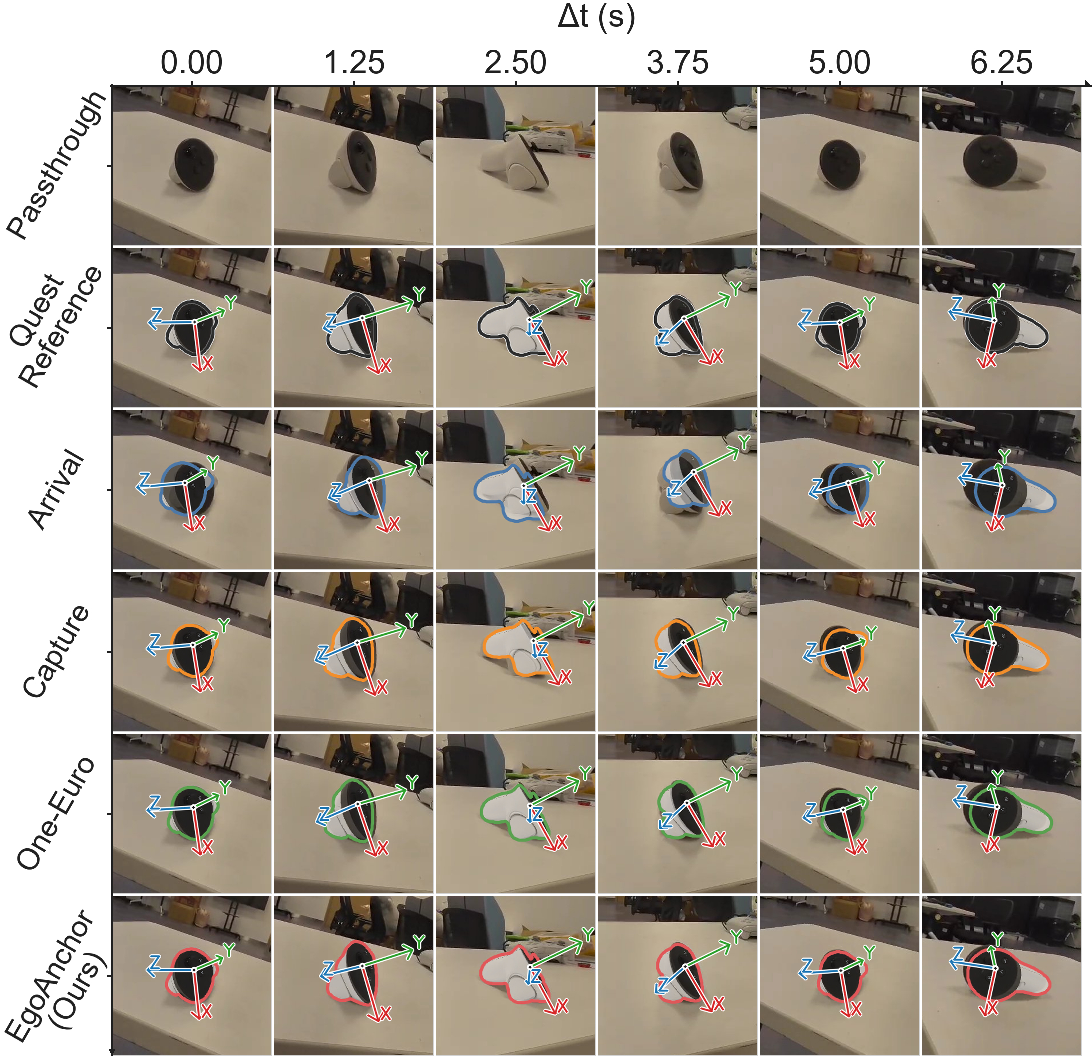
\includegraphics[width=\columnwidth]{figures/replay_grid.pdf}
  \caption{实验一连续序列回放（$\Delta t=0$--$6.25\,\mathrm{s}$，间隔 $1.25\,\mathrm{s}$）。上两行为原始透视图像与 Quest 平台跟踪参考，下四行为 Arrival、Capture、One-Euro、EgoAnchor 在相同采集时刻的锚点投影；轮廓和局部轴表示估计的 6-DoF 锚点，用于比较头动与物体运动下的配准与时间连续性。}
  \label{fig:exp1-replay}
\end{figure}

图~\ref{fig:exp1-replay} 展示了上述定量差异在连续交互过程中的视觉表现：在头部运动阶段，Arrival 与 Capture 出现较明显的空间偏移，One-Euro 减少了部分偏移现象，而 EgoAnchor 保持较低的虚实对齐误差。

\subsection{实验二：消融分析}

实验二各项消融分析均采用独立采集的配对测量数据；每次重复实验先在序列内汇总，再报告跨重复统计量。方括号内为自举 95\% 置信区间，相对变化以配对比值报告。

\begin{figure*}[!t]
  \centering
  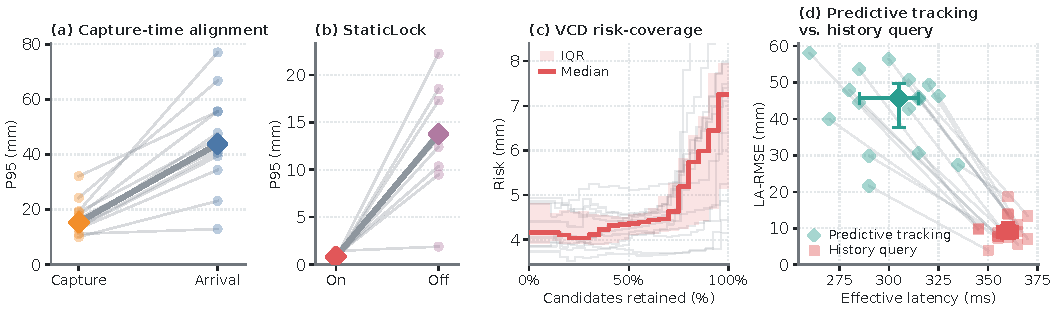
\includegraphics[width=\textwidth]{figures/panels/figure3_exp2_attribution.pdf}
  \caption{实验二模块消融分析：(a) 采用采集时刻或到达时刻相机位姿进行复合时的头动耦合误差 P95 分布；(b) StaticLock 开启或关闭时的头动耦合误差 P95 分布；(c) VCD 风险--覆盖率曲线，灰色细线表示各次重复测量，红线与阴影分别表示跨重复中位数与 IQR；(d) 预测跟踪与历史状态查询在平移通道的有效时延与 LA-RMSE 之间的权衡。在 (a)、(b) 和 (d) 中，灰色细线连接配对测量，彩色大标记与误差棒分别表示中位数与 IQR。}
  \label{fig:exp2-final}
\end{figure*}

图~\ref{fig:exp2-final}(a,b) 分别评估坐标系复合所采用的时间语义以及 StaticLock 的作用。在主动头动条件下，对于同一批相机系候选位姿，采用图像采集时刻的相机位姿进行复合时，头动耦合误差 P95 的中位数为 15.38~mm；采用候选到达时刻的相机位姿时，该误差增至 43.75~mm，配对比值为 2.69 [2.38, 3.00]。这表明，采集时刻对齐可减少头动引起的空间错配。在完整 EgoAnchor 系统上关闭 StaticLock 后，静止状态下的头动耦合误差 P95 从 0.82~mm 增至 13.73~mm，对应配对比值为 17.06 [13.89, 27.52]，说明 StaticLock 能够降低静止阶段的输出波动。

图~\ref{fig:exp2-final}(c) 通过风险--覆盖率曲线评估 VCD 评分与平移误差之间的关系。随着候选接纳比例从高评分区域扩展至低评分区域，选择性风险总体上升。在遮挡条件下，AURC 为 4.79 [4.20, 5.13]~mm，曲线在全覆盖处的风险为 7.25 [5.15, 7.95]~mm。该趋势表明，VCD 评分反映了候选位姿的相对几何可靠性，并可为候选筛选提供排序依据。

图~\ref{fig:exp2-final}(d) 比较了预测跟踪与历史状态查询在响应时延和轨迹保真度方面的差异。预测跟踪的有效时延为 305.00/250.00~ms，低于历史状态查询的 360.00/345.00~ms；但其时延对齐轨迹残差（LA-RMSE）为 45.64~mm/12.21°，高于历史状态查询的 8.93~mm/4.70°。根据配对比值，预测模式下的平移和旋转轨迹残差分别为历史查询模式的 5.46 [4.02, 5.73] 倍和 2.63 [2.44, 2.78] 倍。结果表明，预测跟踪能够降低响应时延，但会增大轨迹估计误差；历史状态查询则具有更高的轨迹几何保真度。

\subsection{实验三：用户实验}

图~\ref{fig:exp3-subjective} 展示了 24 名被试的配对评分结果；12 项评价指标的完整统计结果（包括中位数、Wilcoxon 统计量、Holm 校正后的 $p$ 值及效应量）见补充材料，正文重点报告达到统计学显著性或具有代表性的结果。

\begin{figure*}[!t]
  \centering
  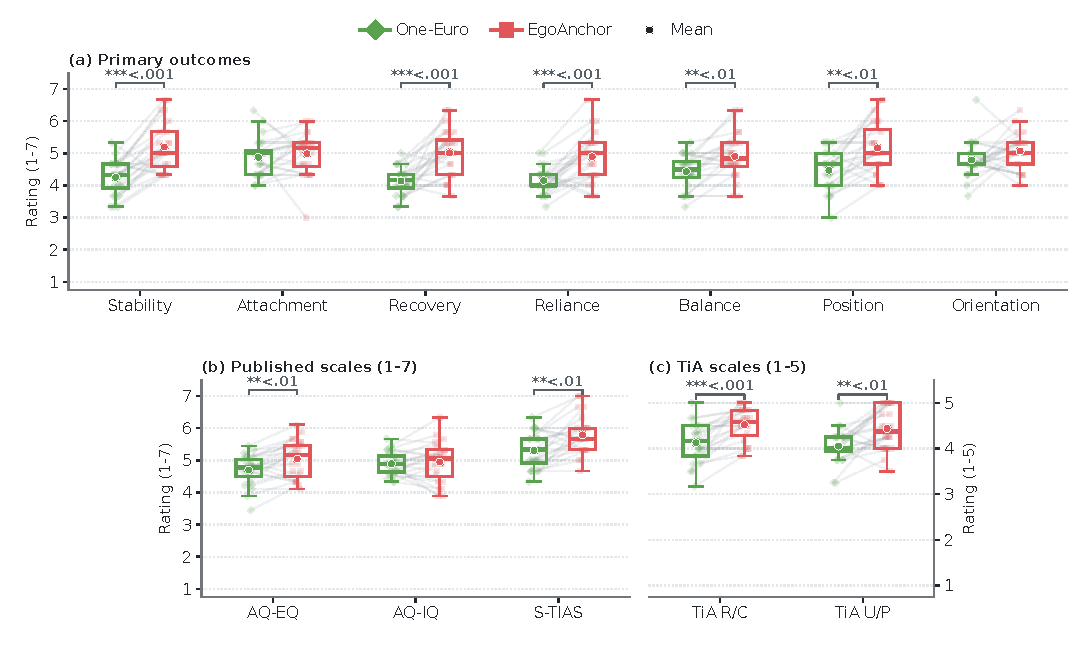
\includegraphics[width=\textwidth]{figures/panels/figure4_exp3_subjective_outcomes.pdf}
  \caption{24 名被试对 One-Euro 与 EgoAnchor 的被试内评价结果：(a) 静止稳定性、运动附着性、姿态一致性和恢复一致性；(b) 位置正确性、依赖意愿以及稳定性--响应性权衡；(c) AQ-EQ、AQ-IQ 与 S-TIAS；(d) TiA 的可靠性/能力（R/C）以及理解性/可预测性（U/P）。每项锚定条目得分与每个 AQ 子量表得分均先在三个物体间取平均；(a)--(c) 使用 7 点量表，(d) 使用 5 点量表。浅色散点与灰色连线表示个体配对评分，箱体、横线和黑点分别表示四分位距、中位数和均值；星号表示经过 Holm 校正后的显著性水平（$^*p_{\mathrm{adj}}<.05$，$^{**}p_{\mathrm{adj}}<.01$，$^{***}p_{\mathrm{adj}}<.001$）。}
  \label{fig:exp3-subjective}
\end{figure*}

\subsubsection{对象锚定体验}

\textbf{静止与恢复阶段。}
七项条目中效应量最大的差异出现在静止与恢复阶段。在静态观察条件下，EgoAnchor 的评分中位数为 5.00 [4.58, 5.67]，高于 One-Euro 的 4.33 [3.92, 4.67]（$W=13.5$，$p_{\mathrm{adj}}<.001$，$r_{\mathrm{rb}}=.90$）。在遮挡移除后，EgoAnchor 的恢复一致性评分为 5.00 [4.33, 5.42]，One-Euro 为 4.17 [3.92, 4.33]，该差异对应七项条目中最大的效应量（$W=6$，$p_{\mathrm{adj}}<.001$，$r_{\mathrm{rb}}=.95$）。

\textbf{持续运动阶段。}
在物体处于持续操纵运动期间，两种系统的主观感知差异明显收窄。运动附着评分在 EgoAnchor（5.17 [4.58, 5.33]）与 One-Euro（5.00 [4.33, 5.08]）之间接近；姿态一致性评分分别为 EgoAnchor 5.00 [4.67, 5.33] 与 One-Euro 4.67 [4.67, 5.00]。经 Holm 校正后两项均未表现出统计学显著差异（附着：$W=67.5$，$p_{\mathrm{adj}}=.267$，$r_{\mathrm{rb}}=.29$；一致：$W=81$，$p_{\mathrm{adj}}=.162$，$r_{\mathrm{rb}}=.41$）。

\textbf{整体锚定判断。}
三项整体评价指标均显示出有利于 EgoAnchor 的统计学显著差异。位置正确性评分为 EgoAnchor 5.00 [4.67, 5.75]、One-Euro 4.67 [4.00, 5.00]（$W=16$，$p_{\mathrm{adj}}=.001$，$r_{\mathrm{rb}}=.85$）；系统依赖意愿为 EgoAnchor 5.00 [4.33, 5.33]、One-Euro 4.00 [4.00, 4.33]（$W=16.5$，$p_{\mathrm{adj}}<.001$，$r_{\mathrm{rb}}=.87$）；稳定性--响应性权衡评分为 EgoAnchor 4.83 [4.58, 5.33]、One-Euro 4.50 [4.25, 4.75]（$W=6$，$p_{\mathrm{adj}}=.003$，$r_{\mathrm{rb}}=.90$）。

\subsubsection{增强质量与信任}

\textbf{增强质量。}
AQ 量表分析表明，系统差异主要体现在虚实融合感（AQ-EQ）而非动态交互质量（AQ-IQ）。EgoAnchor 的嵌入质量评分为 5.17 [4.50, 5.47]，高于 One-Euro 的 4.78 [4.50, 5.03]（$W=32$，$p_{\mathrm{adj}}=.004$，$r_{\mathrm{rb}}=.75$）。交互质量评分的差异则未达到校正后的显著性水平：EgoAnchor 为 5.06 [4.50, 5.33]，One-Euro 为 4.89 [4.64, 5.14]（$W=102.5$，$p_{\mathrm{adj}}=.446$，$r_{\mathrm{rb}}=.19$）。

\textbf{用户信任。}
三项信任指标中，EgoAnchor 均获得更高评价。TiA 可靠性/能力呈现最大效应量（$W=0$，$p_{\mathrm{adj}}<.001$，$r_{\mathrm{rb}}=1.00$）：EgoAnchor 为 4.58 [4.29, 4.83]，One-Euro 为 4.17 [3.83, 4.50]。在理解/可预测性上，EgoAnchor 为 4.38 [4.00, 5.00]，One-Euro 为 4.00 [3.94, 4.25]（$W=32$，$p_{\mathrm{adj}}=.004$，$r_{\mathrm{rb}}=.75$）。S-TIAS 总体信任评分同样显示出显著差异：EgoAnchor 为 5.67 [5.33, 6.00]，One-Euro 为 5.33 [4.92, 5.67]（$W=22.5$，$p_{\mathrm{adj}}=.004$，$r_{\mathrm{rb}}=.79$）。

量表信度检验显示，One-Euro 条件下的 AQ 交互质量（$\alpha=.504$）与 TiA 理解/可预测性（$\alpha=.565$）内部一致性较低，S-TIAS 在两种方法下的 $\alpha$ 亦低于 .70（One-Euro 为 $.672$，EgoAnchor 为 $.697$）。因此，在解释这些量表层面的差异时应保持审慎；完整信度系数见补充材料。

\textbf{总体选择。}
在盲测总体偏好中，62.5\%（15/24）的被试偏好 EgoAnchor，4 人偏好 One-Euro，5 人无明显偏好；在直接信任选择中，18 人选择 EgoAnchor，1 人选择 One-Euro，5 人认为两者相当。被试的偏好强度中位数为 4.00 [3.00, 5.00]，方法区分信心为 6.00 [5.00, 7.00]；实验期间仅 3 人报告轻微不适，无被试中途退出。

\section{讨论}\label{sec:discussion}

\subsection{技术启示}

综合受控测试与主观实验，系统最明确的性能差异来自对图像采集时刻时间语义的显式还原以及对静止状态的专门建模，而非仅依赖帧间自适应平滑。VCD 为候选位姿提供了有效的可靠性排序，历史状态查询则以响应滞后为代价获得了更低的轨迹几何残差。这些客观性能差异与被试在虚实融合感、位置正确性、依赖意愿和交互信任度方面对 EgoAnchor 的更高评价一致。在第一人称动态锚定任务中，实用系统需要将位姿几何、采集时间戳、观测可靠性与异步传输共同组织为可供应用层连续绑定的对象状态。

EgoAnchor 呈现出明确的系统工程取舍：其静态稳定性、遮挡恢复精度与轨迹几何保真度更高，但运动响应时延更长；在持续运动期间，其平移瞬时误差（CT-RMSE）高于直接输出候选的基线。用户实验呈现出一致趋势：EgoAnchor 的优势集中于静止观察、遮挡恢复与整体信任，而在连续操纵阶段，两种方法的主观评分差异未达到统计学显著性。因此，对于物理标注、装配指导和状态监测等重视空间对齐的任务，系统可优先保障稳定性与几何保真度；对于高动态、低时延交互任务，则需进一步优化响应时延。

\subsection{局限与未来工作}

\textbf{对象与三维模型。}
EgoAnchor 目前面向具备已知刚性三维模型的日常物体，其锚定性能受制于目标的视觉可观测性与模型先验质量。严重的视线遮挡、弱纹理表面、高反光或半透明材质以及双目深度估计失效，均会影响分割掩膜与位姿验证的准确性；非刚性形变物体超出本文刚体模型的处理范畴。此外，由于同一三维模型同时参与位姿估计与 VCD 验证，模型自身的几何与尺度偏差会直接引入系统误差。未来工作可研究轻量化的在线几何自适应校准与自动化模型生成流水线。

\textbf{评价参考与跨平台比较。}
本文以平台跟踪控制器为参考的受控基准测试仅在 Meta Quest 3 上完成，尚缺乏跨头显平台的 6-DoF 横向比较。各平台对输入模型的原点、轴向、尺度和预处理要求不同，导致输出位姿定义于不同的对象局部坐标系；此外，传感器配置、时钟同步与跟踪接口也存在差异。Quest 3 控制器虽能提供高精度同步参考，但仍依赖平台原生视觉--惯性解算而非绝对真值。未来可通过统一对象坐标系标定，并引入光学动作捕捉或高精度机械臂，建立更严格的跨平台评估基准。

\textbf{部署与评价基准。}
当前系统依赖外部高性能 GPU 工作站进行感知推理，网络通信与异构计算引入了固有时延；未来可通过模型量化、蒸馏和移动端 NPU 加速，将感知管线轻量化部署至头显设备，以降低端到端时延并提高对高速动态操纵的适应能力。受控基准评测为获得高精度跟踪参考而采用官方控制器；用户实验则选取三种刚性物体，以平衡物体多样性与实验时长。未来可在更多物体类别和异构头显设备上复用静态配准、动态跟随与状态转换响应三类指标，进一步完善动态物体锚定的标准化评测基准~\cite{cheng2024tracking,hu2024applemeta,hu2025xrrealitycheck}。

\section{结论}\label{sec:conclusion}

本文提出 EgoAnchor，一套面向透视混合现实的第一人称零样本动态物体锚定系统。系统将异步相机系观测转换为图像采集时刻的世界系状态，并维护面向渲染管线的可靠对象状态，从而将离散、低频的视觉估计转化为连续、稳定且支持遮挡恢复的空间锚点。受控基准测试与消融分析表明，与基准方案相比，EgoAnchor 的静态配准误差、遮挡恢复误差和轨迹几何残差更低，但运动响应时延更高；24 名被试的被试内用户实验进一步显示，EgoAnchor 在虚实融合感、交互信任度与依赖意愿方面获得了更高评价。

将视觉感知位姿转化为可用对象级空间锚点，不仅依赖底层单帧位姿估计精度，更依赖运行时对时序语义、感知不确定性与状态生命周期的系统性建模。随着开放词表基础模型、三维快速生成技术与移动算力的协同发展，感知--运行时协同架构有望将高保真动态锚定扩展至更多日常物体与自然混合现实交互场景。

\acknowledgments{
  该研究得到中国国家自然科学基金项目（No. 62377004 和 No. 62671062）的资助。OpenAI ChatGPT 仅用于辅助英文翻译和语言润色。作者已审阅并核实所有修改。
}

\bibliographystyle{abbrv-doi-hyperref-narrow}
\bibliography{egoanchor_cn_refs}

\end{document}
